\setchapterpreamble[u]{\margintoc}
\chapter[Signal Flow Graphs ($3^{rd}$ Lecture)]{Signal Flow Graphs}
\labch{lec3}

% Will contain only signal flow graphs, system stability & singularities are shifted to lec 4 ... 

\section{Definitions}
\labsec{sec3.1}

\begin{figure}[h]
	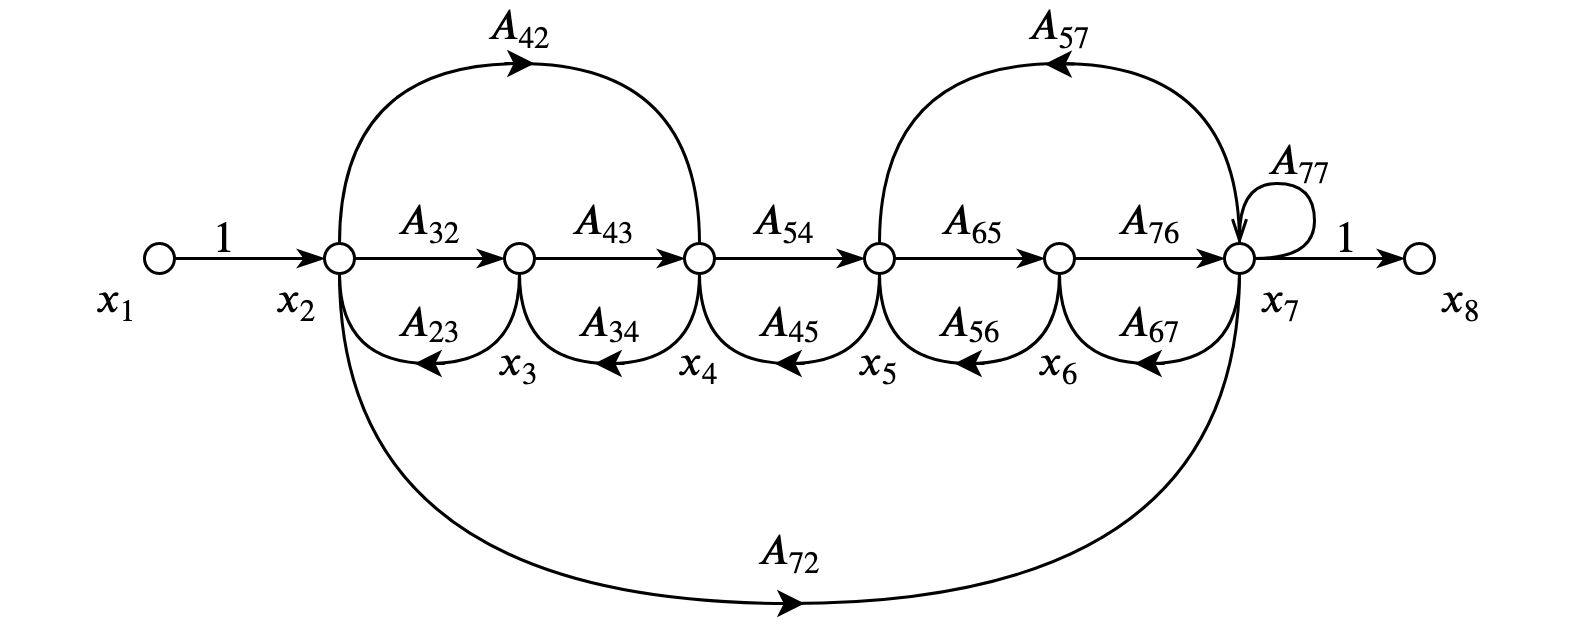
\includegraphics{lec3/Signal Flow}
	\caption{Signal flow general graph.}
\end{figure}

\vspace{-1.25mm}
\subsection[Nodes]{Nodes\linkT{Reference: Feedback control system analysis and synthesis}}

\begin{description}
	\item[Source Nodes]  Represent independent variables and have only outgoing branches. ($x_1$)
	\item[Sink Nodes]  Represent dependent variables and have only incoming branches. ($x_8$)
	\item[Mixed Nodes]  Have both incoming and outgoing branches. ($x_2 \to x_7$)
\end{description}

\vspace{-1.25mm}
\subsection[Paths]{Paths\linkS{http://imtiazhussainkalwar.weebly.com/feedback-control-systems-modeling-and-analysis.html}}

% [+0.42cm] is needed to allign with graphs that is not in margin, so -0.42 is good to allign with text.
% 0.4233401538135892 cm = 12 pt

\begin{description}
	\item[Forward Path]  From the input node to the output node.
		\begin{marginfigure}[-0.4233401538135892cm]
			\includegraphics{lec3/Forwards}
		\end{marginfigure}
	\vspace{2.7 cm}
	
	\item[Feedback loop]  Originates and terminates on the same node.
		\begin{marginfigure}[+0.4233401538135892cm]
			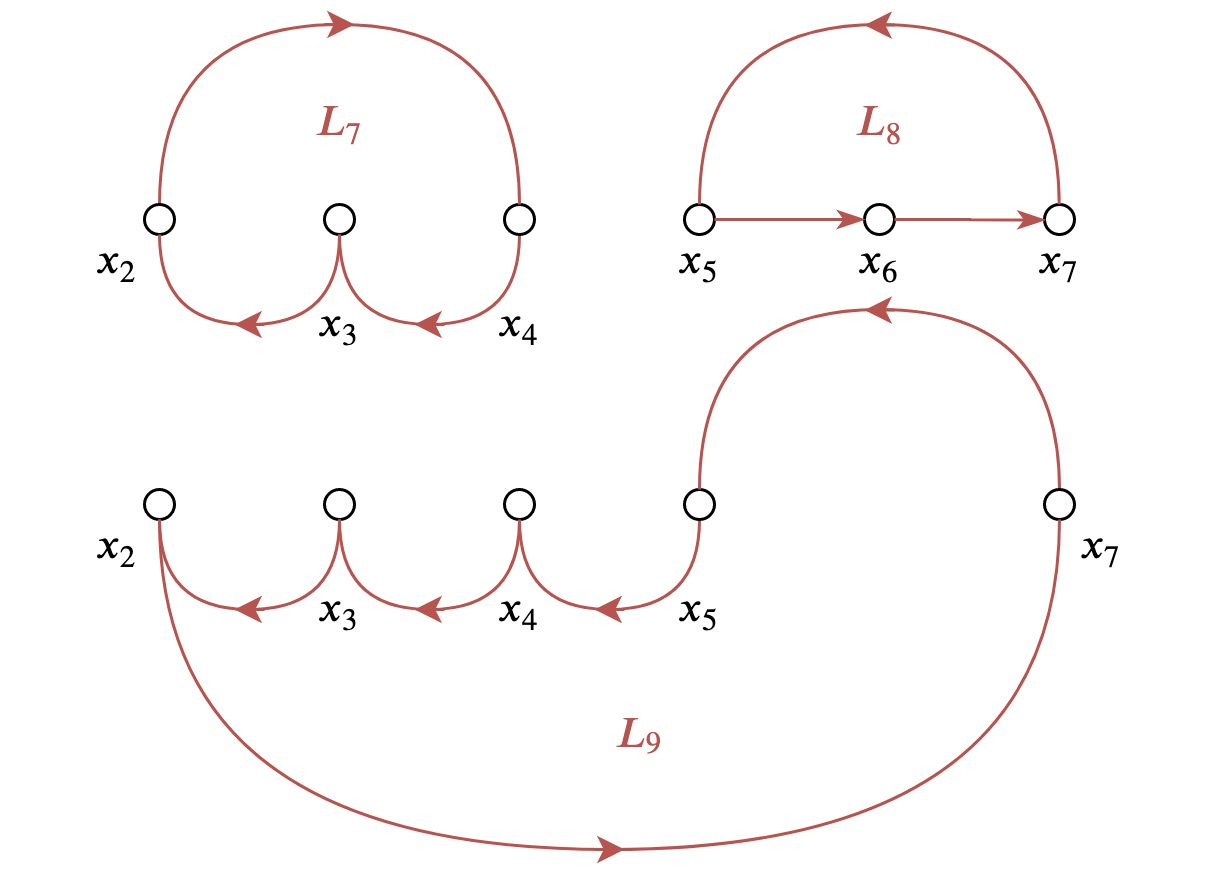
\includegraphics{lec3/Feedbacks - 2} 
		\end{marginfigure}
		\begin{figure}[h]
			\raggedleft
			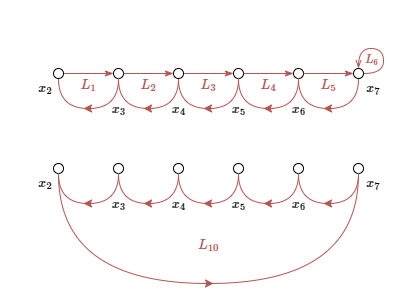
\includegraphics[width=\marginratio\textwidth]{lec3/Feedbacks - 1}
		\end{figure}
	
	\item[Self loop]  A feedback loop consisting of a single branch.
		\begin{figure}[!h]
			\raggedleft
			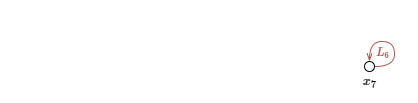
\includegraphics[width=\marginratio\textwidth]{lec3/A loop}
		\end{figure}
		
\end{description}

\subsection{Non-touching loops}

\raggedright
\begin{tabular}{r r r}
	\multicolumn{1}{l}{\textbf{Two at a time}} & \multicolumn{1}{l}{\ \ \ \ \ \textbf{Three at a time}} & \multicolumn{1}{l}{\ \ \ \ \ \textbf{Four at a time}} \\
	\raggedright
	\begin{tabular}{| c | c | c |}
	        \multicolumn{3}{c}{}\\[-1em]
	        $L_1L_3$ & $L_2L_4$ & $L_3L_6$ \\
	        $L_1L_4$ & $L_2L_5$ & $L_4L_6$ \\
	        $L_1L_5$ & $L_2L_6$ & $L_4L_7$ \\
	        $L_1L_6$ & $L_2L_8$ & $L_5L_7$ \\
	        $L_1L_8$ & $L_3L_5$ & $L_7L_8$ \\
	        \multicolumn{3}{c}{}\\[-1em]
	\end{tabular}&
	\raggedright
	\begin{tabular}{|c|}
	        \multicolumn{1}{c}{}\\[-1em]
	        $L_1L_3L_5$ \\
			$L_1L_3L_6$ \\
			$L_1L_4L_6$ \\
			$L_2L_4L_6$ \\
			$ $ \\
	        \multicolumn{1}{c}{}\\[-1em]
	\end{tabular}&\ldots\\
\end{tabular}

\subsection{Gain}
	
\begin{description}
	\item[Path Gain]  Product of branch gains encountered in a path. ($P_3:\ A_{72}$)
	\item[Loop Gain]  Product of the branch gains of the loop. ($L_3:\ A_{54}A_{45}$)
\end{description}

\section[Block to Flow-graph]{Block Diagram to Signal Flow Graph\linkS{https://www.tutorialspoint.com/control_systems/control_systems_signal_flow_graphs.htm}}
\labsec{sec3.3}

\begin{figure}[h]
			\centering
			\includegraphics[width=0.8\textwidth]{lec3/Motor Block Diagram}
			\caption{Motor block diagram.}
\end{figure}

\textbf{Step 1}\ \  Represent all the signals, variables,
summing points and take-off points of block diagram as nodes in signal flow graph.\\
\textbf{Step 2}\ \  Represent the blocks of block diagram as branches in signal flow graph.\\
\textbf{Step 3}\ \  Represent the transfer functions inside the blocks of block diagram as 
gains of the branches in signal flow graph.\sidenote[][]{Connect the nodes as per the block diagram.
If there is connection between two nodes (but there is no block in between),
then represent the gain of the branch as one.}\\[+2em]

\begin{figure}[h]
			\raggedleft
			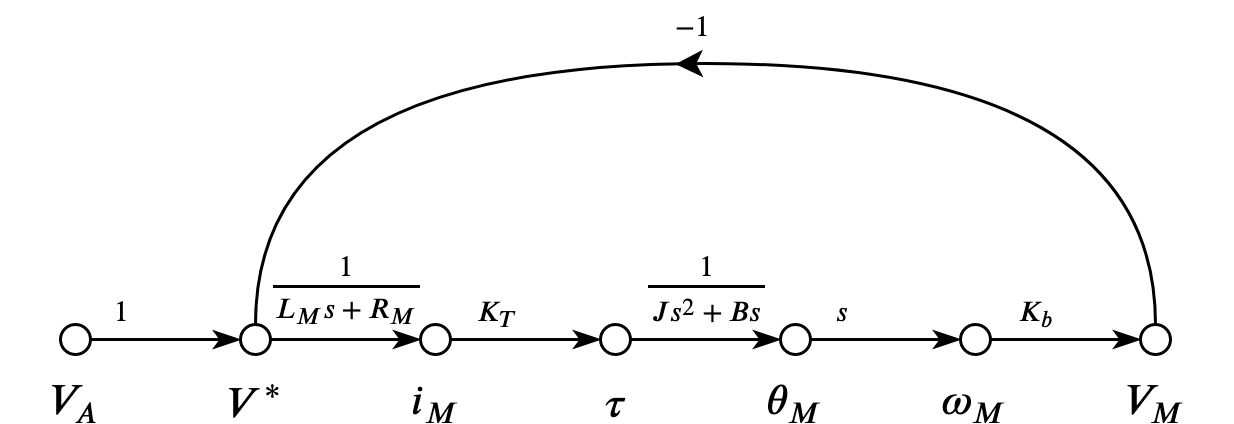
\includegraphics[width=0.7\textwidth]{lec3/Motor Flow Graph}
			\caption{Motor flow-graph diagram.}
\end{figure}

\section[Flow-graph Algebra]{Flow-graph Algebra\linkT{Reference: Feedback control system analysis and synthesis}}
\labsec{sec3.3}

%457		601		463
%601		601		463

%0.4 -> 601
%0.30416 -> 457
%0.30815 -> 463

%0.4	 -> 0.32
%0.30416 -> 0.24333
%0.30815 -> 0.24652

\begin{table}[!h]
	\begin{tabular}{>{\centering\arraybackslash}m{3.5cm} | >{\centering\arraybackslash}m{3.5cm} | >{\centering\arraybackslash}m{3.5cm}}
	       \small $Series\ Paths$ &\small $Parallel\ Paths$ &\small $Node\ Absorption$\\[+1mm]
	       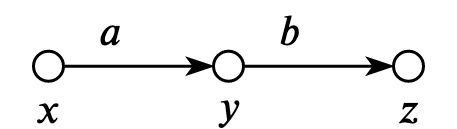
\includegraphics[width=0.24333\textwidth]{lec3/Flow-Graph Algebra - 1}&
	       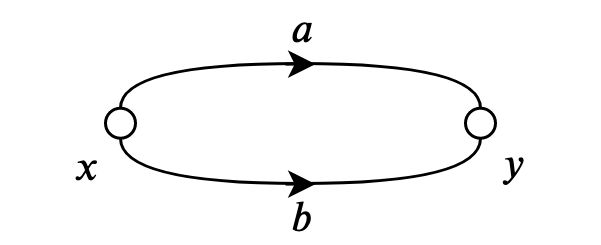
\includegraphics[width=0.32\textwidth]{lec3/Flow-Graph Algebra - 3}&
	       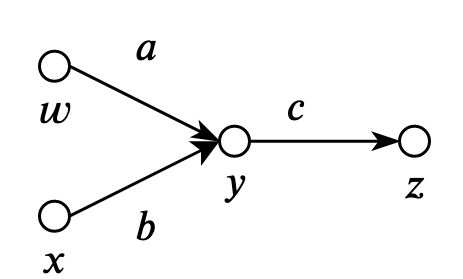
\includegraphics[width=0.24652\textwidth]{lec3/Flow-Graph Algebra - 5}\\
	       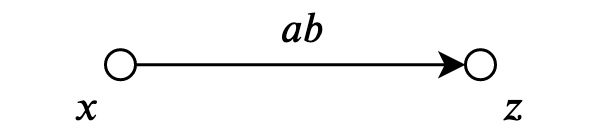
\includegraphics[width=0.32\textwidth]{lec3/Flow-Graph Algebra - 2}&
	       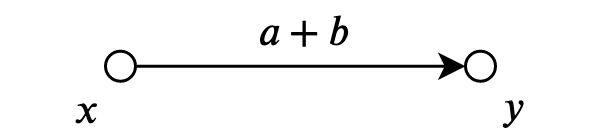
\includegraphics[width=0.32\textwidth]{lec3/Flow-Graph Algebra - 4}&
	       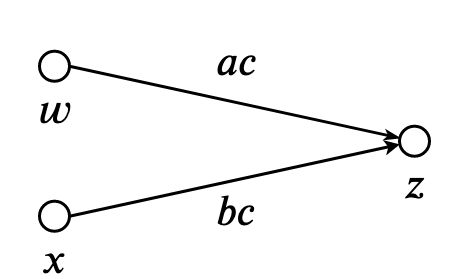
\includegraphics[width=0.24652\textwidth]{lec3/Flow-Graph Algebra - 6}\\
	\end{tabular}
	\caption{Simplification rules.}
\end{table}

\justify
\subsection{Feedback paths}

\begin{marginfigure}[-0.4233401538135892cm]
		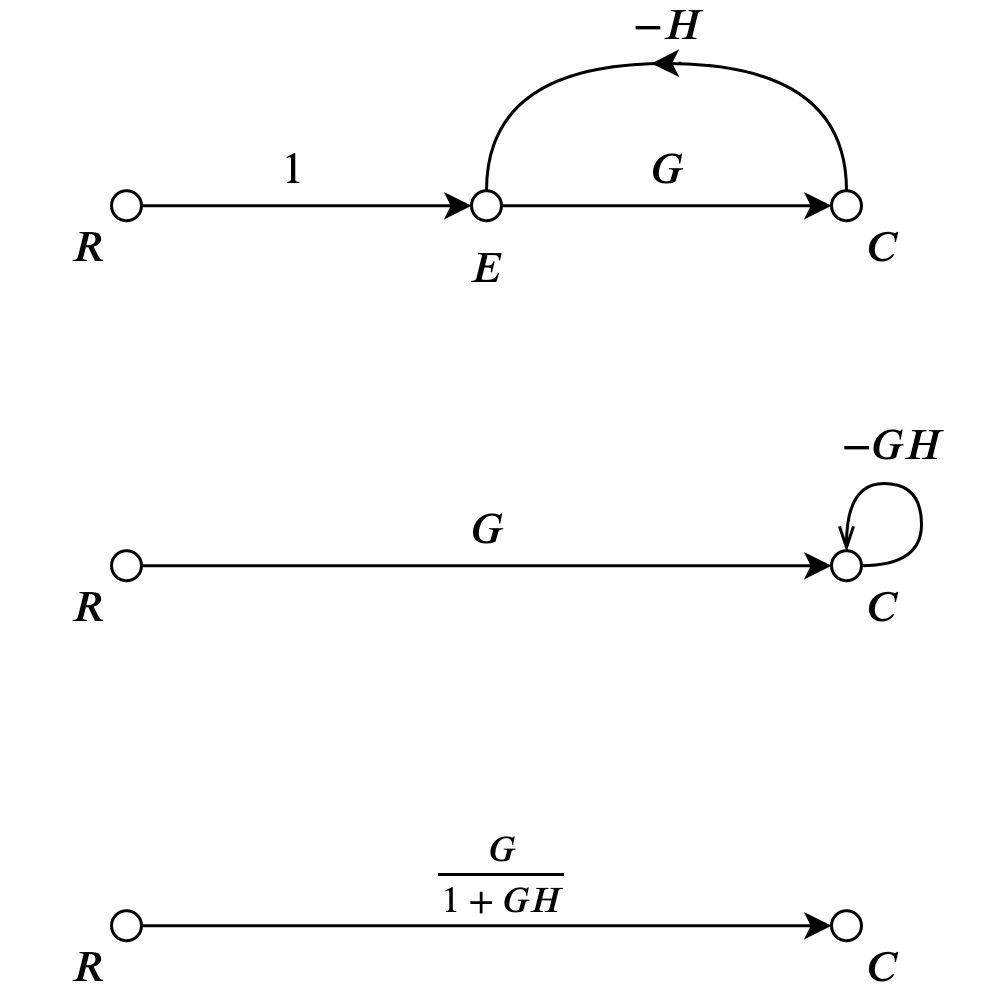
\includegraphics{lec3/Feedback Flow-Graph}
		\caption{Reduction of a feedback path.}
		\labfig{feedbackGraph}
\end{marginfigure}

The equations for the feedback system of \reffig{feedbackGraph} are:\\
\begin{tabular}{p{8cm}p{2cm}}
	&$C=GE$\\
	&$E=R-HC$\\
\end{tabular}
\\
\begin{description}
	\item[Step 1]  The node $E$ can be eliminated to produce a graph with a self-loop.\\[+2.65em]
	\item[Step 2]  The final simplification is to eliminate the self-loop to produce the over-all transmittance.
\end{description}


\section[The Mason Rule]{The Mason Rule\linkS{http://imtiazhussainkalwar.weebly.com/feedback-control-systems-modeling-and-analysis.html}}
\labsec{sec3.4}

The block diagram reduction technique requires successive application of fundamental relationships in order to arrive at the system transfer function.
On the other hand, Mason's rule for reducing a signal-flow graph to a single transfer function requires the application of one formula.


\hspace*{\fill}
\fbox{
	    \parbox{3.5cm}{
	    \large $\dfrac{C(s)}{R(s)}=\dfrac{1}{\Delta}\cdot \displaystyle{\sum_{i=1}^n}\ P_i\ \Delta_i$
    	}
    	\marginnote{
    		\begin{tabular}{ll}
				$\boldsymbol{n}$		&  Number of forward paths.\\
				$\boldsymbol{P_i}$		&  The $i^{th}$ forward path gain.\\
				$\boldsymbol{\Delta}$ 	&  Determinant of the system.\\
				$\boldsymbol{\Delta_i}$ &  Determinant of the $i^{th}$ forward path.\\
    		\end{tabular}
    	}
}


\subsection[Graph determinant]{Graph determinant $\Delta$}

$\boldsymbol{\Delta} = 1-($ sum of all individual loop gains $)+($ sum of the products of the gains of all
possible two loops that do not touch each other $)\ -$ \ldots and so forth with sums of higher
number of non-touching loop gains.

\justify
$\boldsymbol{\Delta_i} =$ value of $\Delta$ for the part of the flow graph that does not touch the $i^{th}$ forward path.
\sidenote{$\Delta_i = 1$ if there are no non-touching loops to the $i^{th}$ path.}



\subsection{Systematic approach}

\begin{marginfigure}
		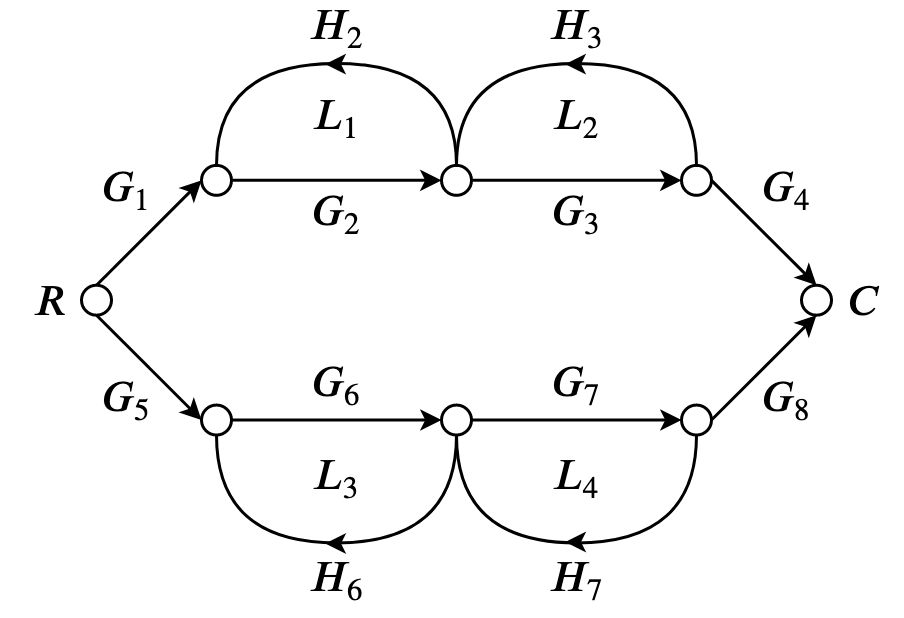
\includegraphics{lec3/Mason Example}
		\caption{Mason rule example.}
\end{marginfigure}

\begin{description}
	\item[Step 1]  Calculate forward path gain $P_i$ for each $i$ forward path.
	\item[Step 2]  Calculate all loops transfer functions.
	\item[Step 3]  Consider non-touching loops 2 at a time, 3 at a time, \ldots etc.
	\item[Step 4]  Calculate $\Delta$ from steps 2 and 3.
	\item[Step 5]  Calculate $\Delta_i$ as portion of $\Delta$ not touching $i$ forward path.
\end{description}

\subsubsection{Step 1}
\begin{tabular}{>{\small\centering\arraybackslash}m{5.35cm}>{\small\centering\arraybackslash}m{5.35cm}}
	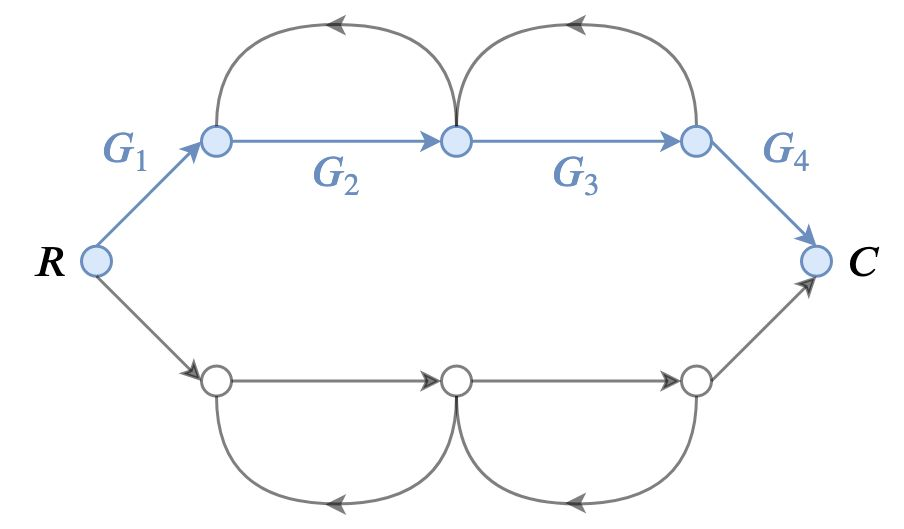
\includegraphics[width=4cm]{lec3/Mason Example - Path1} & 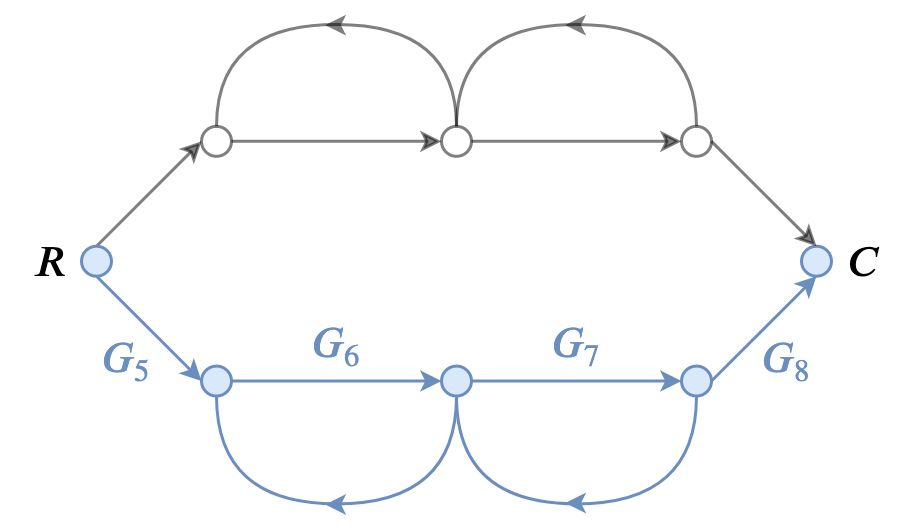
\includegraphics[width=4cm]{lec3/Mason Example - Path2}\\
	&\\[-2mm]
	$P_1 = G_1G_2G_3G_4$ & $P_2 = G_5G_6G_7G_8$ \\
\end{tabular}


\subsubsection{Step 2}

\begin{marginfigure}
		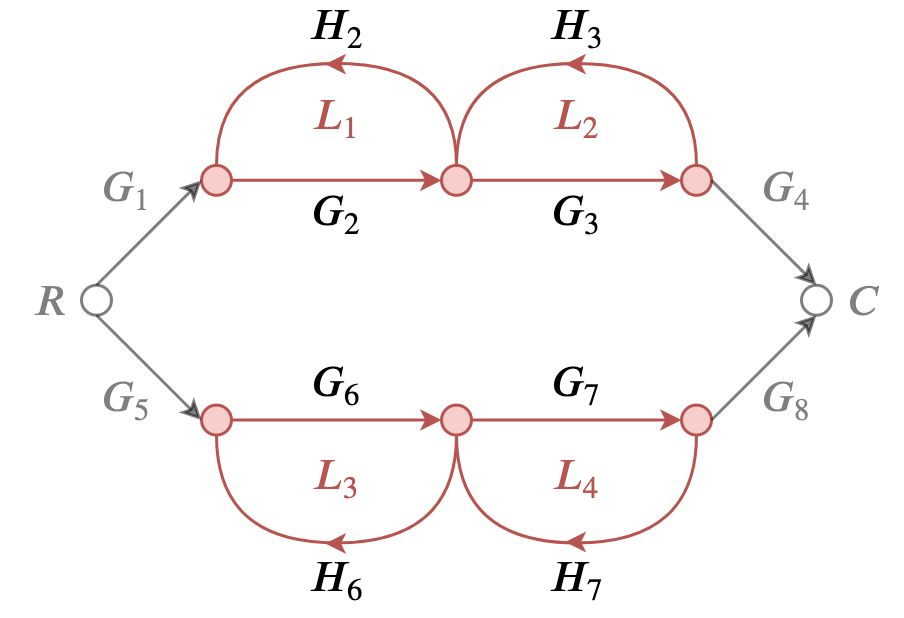
\includegraphics{lec3/Mason Example - Loops Colored}
		\caption{Loops considered.}
\end{marginfigure}

\hspace{1.05cm}
\begin{tabular}{| c |}
			\hline
	        \multicolumn{1}{c}{}\\[-1em]
	        $L_1=G_2H_2$ \\
	        $L_2=G_3H_3$ \\
	        $L_3=G_6H_6$ \\
	        $L_4=G_7H_7$ \\
	        \multicolumn{1}{c}{}\\[-1em]
	        \hline
\end{tabular}


\subsubsection{Step 3}
\raggedright
\begin{tabular}{r r}
	\multicolumn{1}{l}{\textbf{Two at a time}} & \multicolumn{1}{l}{\ \ \ \ \ \textbf{Three at a time}} \\
	\raggedright
	\begin{tabular}{| c |}
	        \multicolumn{1}{c}{}\\[-1em]
	        $L_1L_3$ \\
	        $L_1L_4$ \\
	        $L_2L_3$ \\
	        $L_2L_4$ \\
	        \multicolumn{1}{c}{}\\[-1em]
	\end{tabular}&\ldots\\
\end{tabular}


\subsubsection{Step 4}

\begin{tabular}{l l l}
		$\boldsymbol{\Delta}$ & $=$ & $1-(L_1+L_2+L_3+L_4 )+(L_1 L_3+L_1 L_4+L_2 L_3+L_2 L_4 )$\\[+1em]
		$\boldsymbol{\Delta}$ & $=$ & $1-(G_2H_2+H_3G_3+G_6H_6+G_7H_7)$\\
		&& $\ \ \ +\ (G_2H_2G_6H_6+G_2H_2G_7H_7+H_3G_3G_6H_6+H_3G_3G_7H_7)$\\
\end{tabular}


\subsubsection{Step 5}

\begin{marginfigure}
		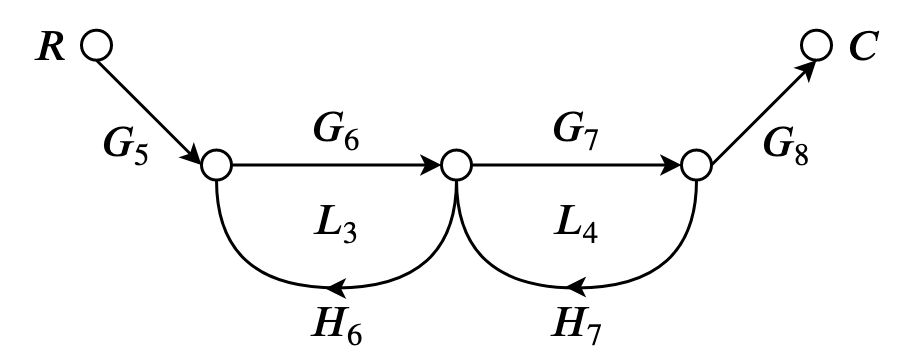
\includegraphics{lec3/Mason Example - Path1 - Eliminated}
		\caption{$P_1$ eliminated.}
\end{marginfigure}

\textit{Eliminate forward path-1:}\\[+1em]
\begin{tabular}{l l l}
		$\boldsymbol{\Delta_1}$ & $=$ & $1-(L_3+L_4)$\\[+1em]
		$\boldsymbol{\Delta_1}$ & $=$ & $1-(G_6H_6+G_7H_7)$\\
\end{tabular}

\vspace{1cm}

\begin{marginfigure}
		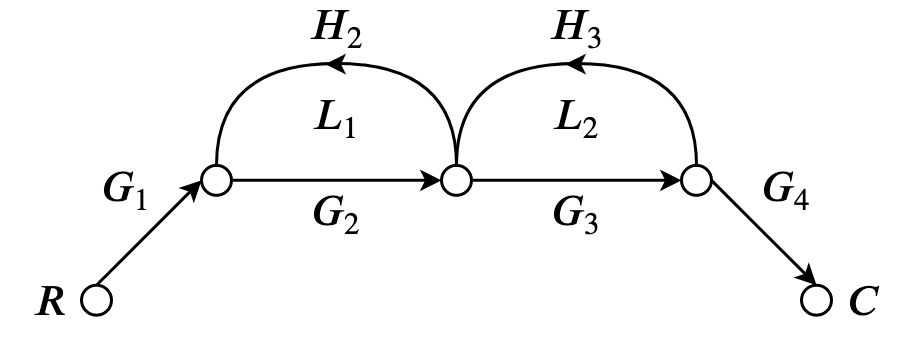
\includegraphics{lec3/Mason Example - Path2 - Eliminated}
		\caption{$P_2$ eliminated.}
\end{marginfigure}

\textit{Eliminate forward path-2:}\\[+1em]
\begin{tabular}{l l l}
		$\boldsymbol{\Delta_2}$ & $=$ & $1-(L_1+L_2)$\\[+1em]
		$\boldsymbol{\Delta_2}$ & $=$ & $1-(G_2H_2+H_3G_3)$\\
\end{tabular}


\subsubsection{Applying Mason's rule}
\begin{tabular}{l l l}
		$\dfrac{\boldsymbol{C(s)}}{\boldsymbol{R(s)}}$ & $=$ & $\dfrac{P_1\Delta_1+P_2\Delta_2}{\Delta}$\\[+1em]
		$\dfrac{\boldsymbol{C(s)}}{\boldsymbol{R(s)}}$ & $=$ & $\dfrac{G_1G_2G_3G_4\ [1-(G_6H_6+G_7H_7)]+G_5G_6G_7G_8\ [1-(G_2H_2+H_3G_3)]}{1-(G_2H_2+H_3G_3+G_6H_6+G_7H_7)+(G_2H_2G_6H_6+G_2H_2G_7H_7+H_3G_3G_6H_6+H_3G_3G_7H_7)}$\\
\end{tabular}